\section{Variable selection using $e$-values}
\label{sec:methodsSection}
We present the details of our methodology in this section. Sections \ref{subsec:DefineModel} and \ref{subsec:meanEvalue} summarize the existing method of $e$-values that performs best subset variable selection in a wide range of statistical models \citep{MajumdarChatterjee17}. We build on this framework in Section \ref{subsec:quantileEvalue}, where we present new results for better detection of weak SNP signals. Section \ref{subsec:BootEvalue} elaborates on the bootstrap implementation of this methodology using the model in \eqref{eqn:LMMeqn}.

\subsection{Models and evaluation maps}
\label{subsec:DefineModel}
In a general modelling situation where one needs to estimate a set of parameters $\bftheta \in \BR^p$ from a triangular array of samples $\cB_n = \{ B_{n1}, \ldots, B_{n k_n} \}$ at stage $n$, any hypothesis or statistical model corresponds to a subset of the full parameter space. Here we consider the model spaces $\bfTheta_{mn} \subseteq \BR^{p}$ in which some elements of the parameter vector have fixed values, while others are estimated from the data. Formally, a generic parameter vector $\bftheta_{mn} \in \bfTheta_{mn}$ consists of entries
%
$$
\theta_{m n j} = \left\{ \begin{array}{ll}
\text{ Unknown } \theta_{m n j} & \text{ for } 
			j \in \cS_{n}; \\
\text{ Known } c_{nj} & \text{ for } j \notin \cS_{n}.
\end{array}
\right.
$$
%
for some $\cS_n \subseteq \{ 1, \ldots, p \}$. Thus the estimable index set $\cS_n$ and fixed elements $\bfc_n = (c_{n j} : j \notin \cS_n)$ fully specify any model in this setup.

At this point, the original framework in \cite{MajumdarChatterjee17} introduces a few concepts to provide a detailed treatment considering a general scenario. For our specific problem, i.e. variable selection, we only require vastly simplified versions of them. We consider sample size $k_n = n$ for all $n$, and assume constant sequences of candidate models: $\cM_n = \cM$ for all $n$. We also drop the subscripts in $\cS_n$ and $\bfc_n$. Thus the `full model', i.e. the model with all covariates is denoted by $\cM_* = (\{ 1, \ldots, p \}, \emptyset)$.

Given data of size $n$, we obtain the full model estimates as minimizers of an estimating equation:
%
\begin{align}\label{eqn:EstEqn}
\hat \bftheta = \argmin_{ \bftheta} \Psi (\bftheta) = \argmin_{ \bftheta } \sum_{i=1}^n \Psi_i (\bftheta, B_i)
\end{align}
%
The only condition we impose on these generic estimating functionals $\Psi_i(.)$ are:

\noindent\textbf{(P1)} The population version of (\ref{eqn:EstEqn}) has a unique minimizer $\bftheta_0$, i.e.
%
\begin{align*}
\bftheta_0 = \argmin_{ \bftheta } \BE \sum_{i=1}^n \Psi_i (\bftheta, B_i)
\end{align*}
%
\noindent\textbf{(P2)} There exist a sequence of positive numbers $a_n \uparrow \infty$ and a $p$-dimensional probability distribution $\BT_0$ such that $a_n (\hat \bftheta - \bftheta_0) \leadsto \BT_0$.
%

We designate $\bftheta_0$ as the {\it true parameter vector}, some elements of which are potentially set to 0. We can now classify any candidate model $\cM$ into one of the two classes: the ones that satisfy $\bftheta_0 \in \bfTheta_m$, and the ones that do not. We denote these two types of models by \textit{adequate} and \textit{inadequate models}, respectively. Given the data and unknown $\bftheta_0$, we want to determine if a candidate model is adequate or inadequate.

For this we need coefficient estimates $\hat \bftheta_m$ corresponding to a model. We do so by just replacing elements of $\hat \bftheta$ not in $\cS$ by corresponding elements of $\bfc$. This means that for the $j^\text{th}$ element, $j = 1, \ldots, p$, we have
%
$$
\hat \theta_{m j} = \left\{ \begin{array}{ll}
\text{ Unknown } \hat \theta_{j} & \text{ for } 
			j \in \cS; \\
\text{ Known } c_{j} & \text{ for } j \notin \cS
\end{array}
\right.
$$
%

We denote the probability distribution of a random variable $\bfT$ by $[\bfT]$. With this notation, we aim to compare the above model estimate distributions with the full model distribution, i.e. $[\hat \bftheta_m]$ with  $[\hat\bftheta]$. For this we define an \textit{evaluation map} function $E: \BR^p \times \tilde \BR^p \raro [0, \infty)$ that measures the relative position of $\hat \bftheta_m$ with respect to $[\hat \bftheta]$. Here $\tilde \BR^p$ is the set of probability measures on $\BR^p$. We assume that $E$ satisfies the following conditions:

\noindent\textbf{(E1)} For any probability distribution $\BG \in \tilde \BR^p$ and $\bfx \in \BR^p$, $E$ is invariant under location and scale transformations:
%
$$
E( \bfx, \BG) = E( a\bfx + \bfb, [a \bfG + \bfb]); \quad a \in \BR \neq 0, \bfb \in \BR^p
$$
%
where the random variable $\bfG$ has distribution $\BG$.

\noindent\textbf{(E2)} The evaluation map $E$ is lipschitz continuous under the first argument:
%
$$
| E( \bfx, \BG) - E( \bfy, \BG) | < \| \bfx - \bfy \|^\alpha; \quad \bfx, \bfy \in \BR^p, \alpha > 0
$$

\noindent\textbf{(E3)}
Suppose $\{ \BY_n \}$ is a tight sequence of probability measures in $\tilde \BR^p$ with weak limit $\BY_\infty$. Then $E( \bfx, \BY_n)$ converges uniformly to $E(\bfx, \BY_\infty)$.

\noindent\textbf{(E4)}
Suppose $\bfZ_n$ is a sequence of random variables such that $\| \bfZ_n \| \stackrel{P}{\raro} \infty$. Then $E( \bfZ_n, \BY_n) \stackrel{P}{\raro} 0$.
\vspace{1em}

For any $\bfx \in \BR^p$ and $[ \bfX ] \in \tilde \BR^p$ with a positive definite covariance matrix $\BV \bfX$, following are examples of the evaluations functions covered by the above set of conditions:
%
\begin{align}\label{eqn:EvaluationExamples}
E_1 (\bfx, [ \bfX]) = \left[ 1 + \left\| \frac{\bfx - \BE \bfX }{ \sqrt { \diag  (\BV \bfX) }}  \right\|^2 \right]^{-1}; \quad
E_2 (\bfx, [ \bfX]) = \exp \left[ - \left\| \frac{\bfx - \BE \bfX }{ \sqrt { \diag  (\BV \bfX) }}  \right\| \right]
\end{align}
%
Data depths \citep{tukey75, zuo00, zuo03} also constitute a broad class of point-to-distribution proximity functions that satisfy the above regularity conditions for evaluation maps. Indeed, \cite{MajumdarChatterjee17} used halfspace depth \citep{tukey75} as evaluation function to perform model selection. However, the conditions (E1) and (E4) are weaker than those imposed on a traditional depth function \citep{zuo00}. Conditions (E2) and (E3) are not required of depth functions in general, but they arise implicitly in several implementations of data depth \citep{MoslerChapter13}. The theoretical results we state here are based on a general evaluation map and not depth functions \textit{per se}. To emphasize this point, in the numerical sections we use the non-depth evaluation functions $E_1$ and $E_2$ as in (\ref{eqn:EvaluationExamples}) above.

%There is no scope of ambiguity in the present analysis about the sample size being $n$, so we drop it in the subscript and have $\BE_m \equiv \BE_{m }$.

\subsection{Model selection using $e$-values}
\label{subsec:meanEvalue}
Depending on the choice of the data sequence $\cB_n$, $E( \hat \bftheta_m, [\hat \bftheta])$ can take different values. For any candidate model $\cM$, we denote the distribution of the corresponding random evaluation map by $\BE_{m n}$. For simplicity we drop the $n$ in its subscript, i.e. $\BE_{m n} \equiv \BE_m$. These distributions are informative of how model estimates behave, and we use them as a tool to distinguish between inadequate and adequate models. Given a single set of samples, we use resampling schemes that satisfy standard regularity conditions \citep{MajumdarChatterjee17} to get consistent approximations of $\BE_{m}$.

We now define a quantity called the \textbf{$e$-value} to compare the different model estimates and eventually perform selection of important SNPs from a multi-SNP model. Loosely construed, any functional of the evaluation map distribution $\BE_{m}$ that can act as model evidence is an $e$-value. For example, \cite{MajumdarChatterjee17} took the mean functional of $\BE_{m }$ (say $\mu (\BE_{m })$) as $e$-value, and proved a result that, when adapted to our setting, states as:

\begin{Theorem}\label{thm:meanThm}
Consider estimators satisfying conditions (P1) and (P2), and an evaluation map $E$ satisfying the conditions (E1), (E2) and (E4). Also suppose that
%
$$
\lim_{n \raro \infty} \mu ( \BY_n ) = \mu ( \BY_\infty) < \infty
$$
%
for any tight sequence of probability measures $\{ \BY_n \}$ in $\tilde \BR^p$ with weak limit $\BY_\infty$. Then as $n \raro \infty$,

\begin{enumerate}
\item For the full model, $\mu (\BE_{* }) \raro \mu_\infty$ for some $0 < \mu_\infty < \infty$;
\item For any adequate model, $| \mu ( \BE_{m } ) - \mu (\BE_{* }) | \raro 0$;
\item For any inadequate model, $ \mu ( \BE_{m }) \raro 0$.
\end{enumerate}
\end{Theorem}

Taking data depths as evaluation functions leads to a further result that $\mu (\BE_{* }) < \mu (\BE_{m })$ for any adequate model $\cM$ and large enough $n$. Following this, non-zero indices of $\bftheta_0$ (say $\cS_0$) can be recovered through a fast algorithm that has these generic steps:

\begin{enumerate}
\item Estimate the $e$-value of the full model, i.e. $\hat \mu (\BE_{* })$, through bootstrap approximation of $\BE_{* }$;
\item For the $j^{\Th}$ predictor, $j=1,\ldots, p$, consider the model with the $j^{\Th}$ coefficient of $\hat \bftheta$ replaced by 0, and get its $e$-value. Suppose this is $\hat \mu (\BE_{-j})$;
\item Collect the predictors for which $\hat \mu (\BE_{-j}) < \hat \mu (\BE_{* })$. Name this index set $\hat \cS_0$: this is the estimated set of non-zero coefficients in $\hat \bftheta$.
\end{enumerate}

\noindent As $n \raro \infty$, the above algorithm provides consistent model selection, i.e. $\BP ( \hat \cS_0 = \cS_0) \raro 1$, with the underlying resampling distribution having mean 1 and variance $\tau_n^2$ such that $\tau_n \raro \infty, \tau_n/\sqrt n \raro 0$ as $n \raro \infty$ \citep{MajumdarChatterjee17}.

\subsection{Quantiles of $\BE_{m }$ as $e$-values}
\label{subsec:quantileEvalue}
%The above formulation of $e$-values leads to favorable finite sample results compared to several existing covariate selection techniques in linear and linear mixed models \citep{MajumdarChatterjee17}. However, its performance is dependent on the relative magnitude of the non-zero coefficients to the random error term, i.e. the signal-to-noise ratio (SNR). 
When true signals are weak, the above method of variable selection leads to very conservative estimates of non-zero coefficient indices, i.e. a large number of false positives in a sample setting. This happens because even though at the population level $\mu (\BE_{* })$ separates the population means of inadequate model sampling distributions and those of adequate models, for weak signals bootstrap estimates of adequate model distributions almost overlap with those of the full model.

Figure \ref{fig:figSmallhSim} demonstrates this phenomenon in our simulation setup. Here we analyze data on 250 families with monozygotic twins, each individual being genotyped for 50 SNPs. Four of these 50 SNPs are causal: each having a heritability of $h/6\%$ with respect to the total error variation present. The four panels show density plots of $\hat \BE_{-j}$ for $j = 1, \ldots, p$, as well as $\hat \BE_{* }$: based on resampling schemes with four different values of the standard deviation parameter $s \equiv s_n = \tau_n / \sqrt n $. While smaller values of $s$ are able to separate out the bootstrap estimates of $\BE_{-j}$ for inadequate and adequate models, all the density plots are to the left of the curve corresponding to the full model.

\begin{figure}
\centering
\includegraphics[height=.22\textheight]{{"../Codes/plot_h0.05_tau2"}.pdf}\\
\includegraphics[height=.22\textheight]{{"../Codes/plot_h0.05_tau3"}.pdf}\\
\includegraphics[height=.22\textheight]{{"../Codes/plot_h0.05_tau6"}.pdf}\\
\includegraphics[height=.22\textheight]{{"../Codes/plot_h0.05_tau10"}.pdf}
\caption{Density plots of bootstrap approximations for $\BE_{* }$ and $\BE_{-j}$ for all $j$ in simulation setup, with $s = 0.2, 0.3, 0.6, 1$}
\label{fig:figSmallhSim}
\end{figure}

However, notice that the inadequate and adequate model distributions have different tail behaviors for smaller values of $s$, and setting an appropriate upper threshold to tail probabilities for a suitable fixed quantile of these distributions with respect to the full model distribution can possibly provide a better separation of the two types of distributions. For this reason we use tail quantiles as $e$-values.

We denote the $q^{\Th}$ population quantile of $\BE_{m }$ by $c_{q} ( \BE_{m } ) $. Then we have equivalent results to Theorem \ref{thm:meanThm} as $n \raro \infty$:

\begin{Theorem}\label{thm:quantileThm}
Given that the estimator $\hat \bftheta$ satisfies conditions (P1) and (P2), and the evaluation map satisfies conditions (E1)-(E4), we have
%
\begin{align}
& c_{q} ( \BE_{* } ) \raro c_{q,\infty} < \infty \label{evalEqn1}\\
& | c_{q} ( \BE_{m } ) - c_{q} ( \BE_{* } ) | \raro 0 \text{ when } \cM \text{ is adequate}\label{evalEqn2}\\
& c_{q} ( \BE_{m } ) \raro 0 \text{ when } \cM \text{ is inadequate} \label{evalEqn3}
\end{align}
\end{Theorem}
%
%\noindent These results are proved by taking a similar approach as that of proving Theorem \ref{thm:meanThm}. We do this in the supplementary material.

When the $q^\text{th}$ quantile is taken as the $e$-value instead of the mean, we set a lower detection threshold than the same functional on the full model, i.e. choose all $j$ such that $c_q (\BE_{-j}) < c_{q t} (\BE_{*}), 0 < t < 1$ to be included in the model. The choice of $t$ potentially depends on several factors such as the value of quantile evaluated, the statistical model used, sample size and degree of sparsity of parameters in the data generating process. We illustrate this point on simulated data in Section~\ref{sec:SimSection}.

\subsection{Bootstrap procedure}
\label{subsec:BootEvalue}
We use generalized bootstrap \citep{ChatterjeeBose05} to obtain approximations of the sampling distributions $\BE_{-j}$ and $\BE_*$. It calculates bootstrap equivalents of the parameter estimate $\hat \bftheta$ by minimizing a version of the estimating equation in (\ref{eqn:EstEqn}) with random weights:
%
\begin{align}
\hat \bftheta_w = \argmin_{ \bftheta} \sum_{i=1}^n \BW_{i} \Psi_i  ( \bftheta, B_i)
\end{align}
%
The resampling weights $(\BW_{1}, \ldots, \BW_{n})$ are non-negative exchangeable random variables chosen independent of the data, and satisfy the following conditions:
%
\begin{eqnarray}
\BE \BW_1  = 1; \quad
\BV \BW_1  = \tau_{n}^{2} \uparrow \infty; \quad
\tau_n^{2} 
%%= o ( \{min} ( a_n^{2}, n))
= o ( a_n^{2})\label{eq:ResamplingweightBW}\\
\BE W_{1} W_{2} = O (n^{-1}); \quad
\BE W_{1}^{2} W_{2}^{2} \raro 1; \quad
\BE W_{1}^{4} < \infty \label{eq:ResamplingweightW}
\end{eqnarray}
%
with $W_i := (\BW_i - 1)/ \tau_n; i = 1, \ldots, n$ being the centered and scaled resampling weights. Under standard regularity conditions on the estimating functional $\Psi(.)$ \citep{ChatterjeeBose05, MajumdarChatterjee17} and conditional on the data, $(a_n/\tau_n) (\hat \bftheta_w - \hat \bftheta)$ converges to the same asymptotic distribution as $a_n ( \hat \bftheta - \bftheta_0 )$, i.e. $\BT_0$.

We use empirical quantiles of the full model bootstrap samples as the quantile $e$-value estimates. Specifically, we go through the following steps:
%
\begin{enumerate}
\item Fix $q,t \in (0,1)$;

\item Generate two independent set of bootstrap weights, of size $R$ and $R_1$, and obtain the corresponding approximations to the full model sampling distribution, say $[ \hat\bftheta_{r} ]$ and $[ \hat\bftheta_{r_1} ]$;

\item For $j = 1,2,\ldots p$ and estimate the $e$-value of the $j^{\Th}$ predictor as the empirical $q^{\Th}$ quantile of $\hat \BE_{-j} := [ E( \hat \bftheta_{r,-j}, [ \hat \bftheta_{r_1}]) ]$, with $\hat \bftheta_{r,-j}$ obtained from $\hat \bftheta_{r}$ by replacing the $j^{\Th}$ coordinate with 0;

\item Estimate the set of non-zero covariates as
%
$$
\hat \cS_{0} = \lbrace j: c_q (\hat\BE_{-j}) <  c_{q t} (\hat\BE_{*}) \};
$$
\end{enumerate}
%
Conditions (\ref{eq:ResamplingweightBW}) and (\ref{eq:ResamplingweightW}) on the resampling weights ensure bootstrap-consistent approximation of the evaluation map quantiles:
%
%

\begin{Theorem}\label{thm:bootThm}
Given the estimator $\hat \bftheta$ and evaluation map $E$ in Theorem~\ref{thm:quantileThm}, and a generalized bootstrap scheme satisfying (\ref{eq:ResamplingweightBW}) and (\ref{eq:ResamplingweightW}), we get
\begin{align}
& | c_{q} ( \hat \BE_{m } ) - c_{q} ( \hat \BE_{* } ) | \stackrel{P_n}{\raro} o_P(1) \text{ when } \cM \text{ is adequate}\label{bootevalEqn2}\\
& c_{q} ( \hat \BE_{m } ) \stackrel{P_n}{\raro} o_P(1) \text{ when } \cM \text{ is inadequate} \label{bootevalEqn3}
\end{align}
%
where $P_n$ is probability conditional on the data.
\end{Theorem}

Generalized bootstrap covers a large array of resampling procedures, for example the $m$-out-of-$n$ bootstrap and a scale-enhanced version of the bayesian bootstrap. %, as well as the residual-based wild bootstrap \citep{Mammen93}.
 Furthermore, given that $\Psi_i(.)$ are twice differentiable in a neighborhood of $\bftheta_0$ and some other conditions in \cite{ChatterjeeBose05}, there is an approximate representation of $\hat \bftheta_w$:
%
\begin{align}\label{eqn:BootEqn}
\hat\bftheta_w = \hat\bftheta - \frac{ \tau_n}{a_n} \left[ \sum_{i=1}^n W_i \Psi_i'' (\hat \bftheta, B_i) \right]^{-1}
\sum_{i=1}^n W_i \Psi_i' (\hat \bftheta, B_i) + \bfR_{wn}
\end{align}
%
with $\BE_w \| \bfR_{w n} \|^2 = o_P(1)$.

Given the full model estimate $\hat \bftheta$, and the score vectors $ \Psi_i' (\hat \bftheta, B_i)$ and hessian matrices $ \Psi_i'' (\hat \bftheta, B_i)$, (\ref{eqn:BootEqn}) allows us to obtain multiple copies of $\hat \bftheta_w$ through Monte-Carlo simulation of several arrays of bootstrap weights. This bypasses the need to fit the full model for each bootstrap sample, resulting in extremely fast computation of $e$-values.

We adapt the approximation of (\ref{eqn:BootEqn}) to the LMM in (\ref{eqn:LMMeqn}). We first obtain the maximum likelihood estimates $\hat \bfbeta_g, \hat \sigma_a^2, \hat \sigma_c^2, \hat \sigma_e^2$ through fitting the LMM. Then we replace the variance components in (\ref{eqn:partsOfV}) with corresponding estimates to get $\hat \bfV_i$ for $i^{\Th}$ pedigree, and aggregate them to get the covariance matrix estimate for all samples:
%
$$
\hat \bfV = \diag ( \hat \bfV_1, \ldots, \hat \bfV_m )
$$
%
We take $m$ random draws from Gamma$(1,1) - 1$, say $\{ w_{r1}, \ldots, w_{rm} \}$, as resampling weights in (\ref{eqn:BootEqn}), using the same weight for all members of a pedigree. Consequently, the bootstrapped coefficient estimate $\hat \bfbeta_{r g}$ has the following representation:
%
\begin{align}
\hat \bfbeta_{r g} & \simeq \hat \bfbeta_g + \frac{ \tau_n}{\sqrt n} ( \bfG^T \hat \bfV^{-1} \bfG )^{-1}
\bfW_r \bfG^T \hat \bfV^{-1} ( \bfy - \bfG \hat \bfbeta_g)
\end{align}
%
with $\bfG = ( \bfG_1^T, \ldots, \bfG_m^T )^T$ and $\bfW_r = \diag (w_{r1} \bfI_4, \ldots, w_{r m} \bfI_4 )$. Finally we repeat the procedure for two independent sets of resampling weights, say of sizes $R$ and $R_1$, to obtain two collections of bootstrapped estimates $\{ \hat \bfbeta_{1g}, \ldots, \hat \bfbeta_{Rg} \}$.

%We now take a closer look at the evaluation map distributions corresponding to reduced model coefficient estimates, in order to better detect the weak signals we are dealing with here and reduce the number of false positives. Carrying over notations from \ref{chapter:Chapter-evalue}, recall that the model formed by dropping the $j$-the index is denoted by $\cM_{-j}$, and we are going to inspect $\BD_{-j}$, the distribution of $D( \hat \bfbeta_{-j}, [\hat \bfbeta] ) $ by comparing it with $\BD :=$ distribution of $D( \hat \bfbeta, [\hat \bfbeta] ) $. Also define by $\mu(.)$ the mean operator on the corresponding distributions.

%Recall from \ref{chapter:Chapter-evalue} that we approximate the above distributions and the final $e$-value through resampling. The quality of approximation depends on the variance parameter $\tau_n^2$, and as seen in the simulation section, on the type of bootstrap scheme used (moon/ gamma/ generalized). Because of the high-computational overhead of the \texttt{regress} procedure, we shall use the parametric generalized bootstrap scheme here. We would also like to emphasize that all observations in this subsection are entirely empirical and from controlled simulation setups, and further studies are warranted to theoretically characterize such behavior.

%We denote by $\hat \BD_{-j} (\tau)$ and $\hat\BD (\tau)$ the approximations of $\BD_{-j}$ and $\BD$, respectively, using a generalized bootstrap scheme with standard deviation $\tau_n \equiv \tau$. According to theorem \ref{Theorem:ModelScore}, in case $\BD_{-j}$ is an inadequate model distribution, the mean of $\hat \BD_{-j} (\tau)$ goes to 0 in probability for an intermediate rate of the bootstrap standard deviation. As $\tau$ increases, all reduced model distributions approach $\hat\BD (\tau)$. However, depending on the magnitude of signals at the non-zero indices, we observe that this behavior follows two different regimes. We demonstrate this using the simulation setup we elaborate on later in the chapter. In the plots below, $h$ represents the relative magnitude of non-zero entries in the coefficient vector: for which we consider two choices, $h=5$ and $h=0.05$.

%\begin{figure}
%\centering
%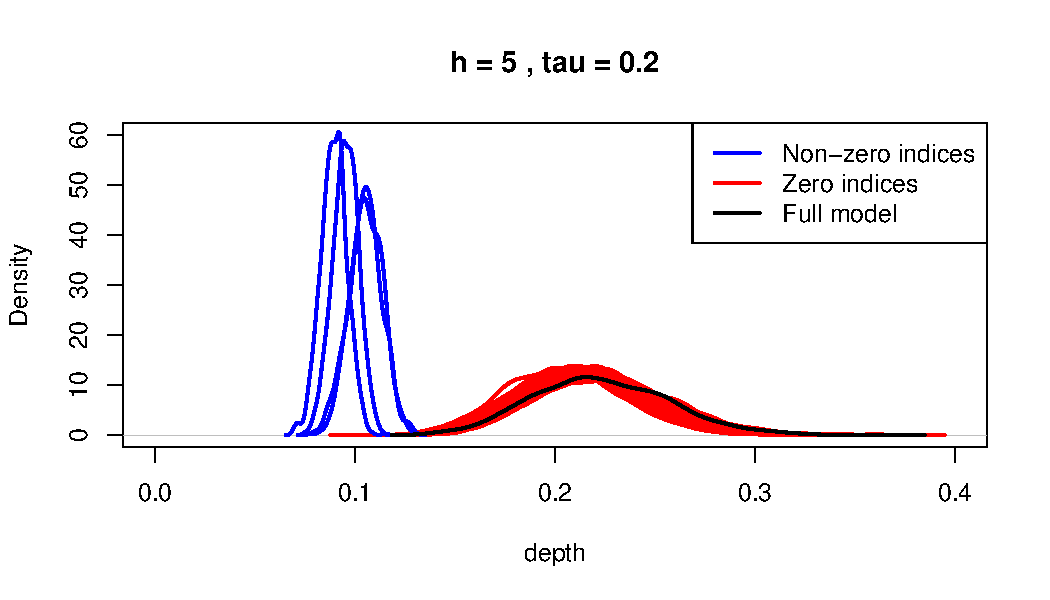
\includegraphics[height=.22\textheight]{../Codes/plot_h5_tau2}\\
%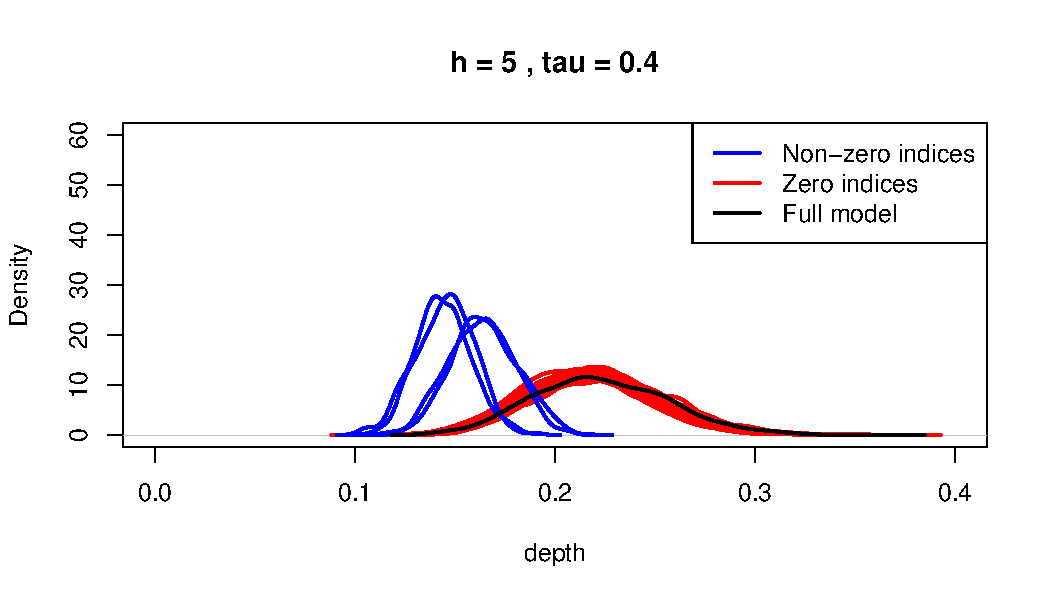
\includegraphics[height=.22\textheight]{../Codes/plot_h5_tau4}\\
%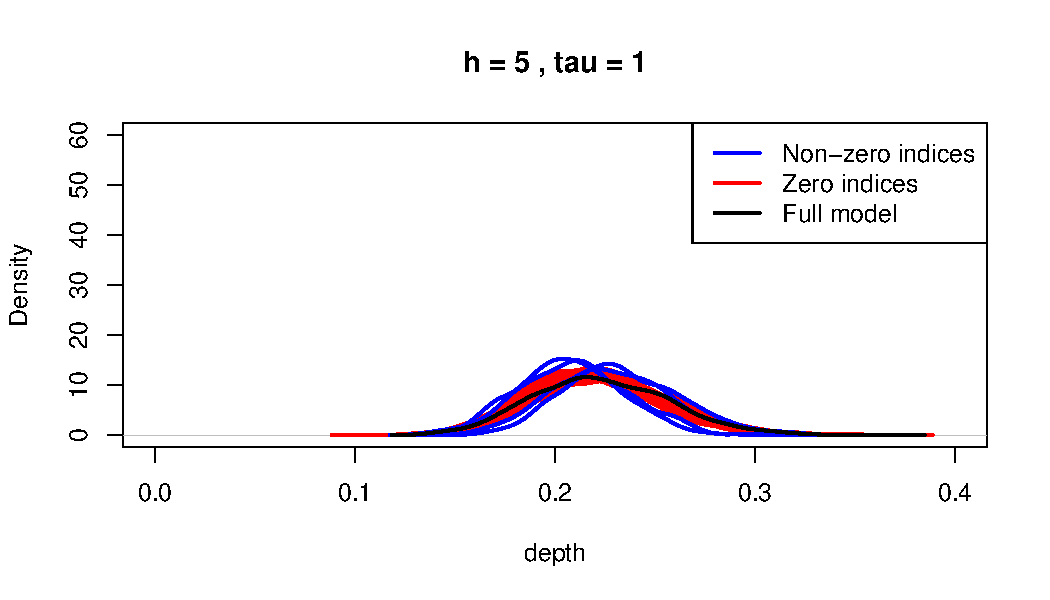
\includegraphics[height=.22\textheight]{../Codes/plot_h5_tau10}\\
%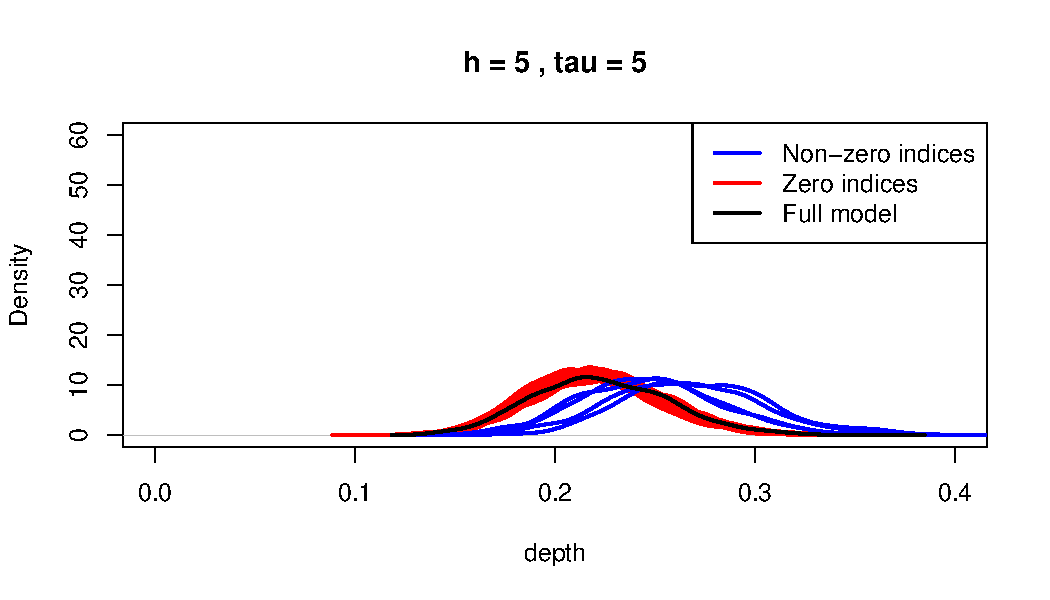
\includegraphics[height=.22\textheight]{../Codes/plot_h5_tau50}
%\caption{Density plots for $\hat \BD(\tau)$ and $\hat \BD_{-j}(\tau)$ for all $j$ in simulation setup, with signal parameter $h=5$ and bootstrap standard deviations $\tau = 0.2, 0.4, 1, 5$}
%\label{fig:figLargeTau1}
%\end{figure}

%\paragraph{(a) Large signal regime ($h=5$: \ref{fig:figLargeTau1})} When $\BD_{-j}$ corresponds to an inadequate model, i.e. the $j$-th coefficient of the true parameter vector is non-zero, for small values of $\tau$ we can clearly distinguish this distribution from that of $\hat\BD (\tau)$ in their density plots. As $\tau$ increases, the inadequate model distributions seem to have more and more positive bias. However, when $j$ is a non-essential covariate, the reduced distributions are close to $\hat \BD(\tau)$ for all values of $\tau$.
%
%\paragraph{(b) Small signal regime ($h=0.05$: \ref{fig:figLargeTau2})} When the actual signal in $\beta_j$ is weak, the inadequate reduced model distributions still approach $\hat \BD(\tau)$ as $\tau$ goes up but stabilize at the full model distribution instead of passing it for very large $\tau$ ($\tau=5$ here). However the adequate model distributions seem to exhibit a similar behavior: albeit staying to the left of inadequate model density plots in general.

%This increased ambiguity of reduced model distributions for small signals make it difficult to distinguish between two types of model distributions using the mean operator, which ends up being very conservative in the second case. For this reason we consider the usage of a different summarizing function that will be able to capture the differentiate between the two types of reduced model distributions across a broader range of the signal-to-noise ratio, specifically by setting a lower detection threshold than the same operator on the full model distribution. Here we focus on a specific alternate formulation of the $e$-value that is based on a tail quantile of $\hat \BD_{-j} (\tau)$:
%%
%\begin{align}
%e_q (\cM_{-j} | \tau) = q \text{-th quantile of } \hat \BD_{-j} (\tau)
%\end{align}
%%
%for some fixed $q \in (0,1)$. Notice that for any $q$, the quantity $e_q (\cM_{-j} | \tau)$ is conditional on the bootstrap standard deviation parameter $\tau$.
%
%The motivation behind this is the observation  
%Also note that we still retain the main flavor of the $e$-values method, by training only the full model and then use Monte Carlo resampling to compute $e_q (\cM_{-j} | \tau)$ for all $j$ and a range of $\tau$.